%!TEX root = ../book.tex

% ******************************* Part: Relational Databases ****************************

%this is a overarching PART that can be replicated to change overarching areas in the book
\part{Relational Databases}
\label{part:relationaldatabases}
This \lcnamecref{part:relationaldatabases} of the book teaches the basics of relational databases. It will walk you through the basics of relational databases, and how to design a database from scratch. After this, it will teach you how to create ER and EER diagrams, and how to design a database from an ER model. Finally, it will teach you how to normalize a database to the 4th normal form.

% ******************************* Chapter: Introduction ****************************
\chapter{Introduction}
\label{chap:relational:introduction}
This chapter introduces the fundamental concept of databases. It begins with a clear definition of what databases are, providing an overview of their purpose and significance in storing and managing information. The chapter then guides the reader through the process of database creation, highlighting the key steps involved from design to deployment. Essential components of a database, such as tables, fields, keys, and relationships, are explained in a concise manner. This chapter serves as a foundational starting point for those new to databases, offering a clear understanding of their basic structure and components.

\section{What is a database?}
A database is a place data can be stored in large quantities in a structured way. It is a collection of data that is organized in such a way that it can be easily accessed, managed and updated. A key property of databases is also the fact that they are persistent, meaning that the data is stored on a physical medium, such as a hard drive, and is not lost when the computer is turned off, as well as the fact that it allows you to create dynamic queries, meaning that you can ask complex questions of the data.

A database is a structured and organized collection of data that serves as a centralized repository for storing, managing, and retrieving information. Its primary purpose is to efficiently store and manipulate data to support various applications and processes. At its core, a database consists of two key elements:

\begin{enumerate}
    \item Data: Data is the fundamental building block of a database. It represents the information that needs to be stored, and it can take various forms, including text, numbers, dates, and multimedia. Data is organized into tables, records, and fields, with each table containing related information and each record representing a distinct unit of data, while fields hold specific attributes or properties of that data.
    \item Database Management System (DBMS): The DBMS is the software that facilitates interactions with the database. It acts as an intermediary between users or applications and the actual data storage. The DBMS provides essential functionalities such as data retrieval, insertion, updating, and deletion, as well as enforcing data integrity, security, and ensuring efficient data access through query processing. It also manages concurrency control to ensure that multiple users can work with the database simultaneously without data conflicts.
    \item Querying: is another key element of databases. Querying involves the ability to retrieve specific information from the database based on predefined criteria or user-defined queries. It allows users to filter, search, and analyze data to extract meaningful insights. Querying is facilitated through a query language (e.g., SQL for relational databases) or query APIs (Application Programming Interfaces) that enable users and applications to interact with the database and request specific subsets of data. The querying aspect is crucial because it empowers users to access and manipulate data in a flexible and efficient manner, making databases highly versatile for various applications, including research, reporting, decision-making, and data analysis. Whether it's retrieving a list of products from an inventory database or extracting research findings from a scientific database, querying capabilities are fundamental to harnessing the full potential of a database's stored information.
\end{enumerate}

A database, regardless of its specific type, serves as a vital tool for efficiently organizing and manipulating data, making it accessible and useful for various purposes, including research, analysis, and application development.

\section{What exactly is a relational database?}
A relational database is a specific type of database management system (DBMS) that organizes and manages data using a structured approach based on the principles of relational algebra. It differs from the broader term "database" in several key ways:

\begin{enumerate}
    \item Data Structure: In a relational database, data is structured into tables, where each table consists of rows (tuples) and columns (attributes, properties). This tabular format is highly organized and allows for the representation of complex relationships between data entities. Each table represents a distinct entity or concept, and the relationships between these tables are defined through keys, such as primary keys and foreign keys.
    \item Data Integrity: Relational databases enforce data integrity through a set of rules and constraints. These constraints ensure that data remains consistent and accurate. For example, primary keys enforce the uniqueness of each record in a table, while foreign keys establish relationships between tables, maintaining referential integrity. These mechanisms help prevent data anomalies and maintain data quality.
    \item SQL Language: Relational databases use the Structured Query Language (SQL) as the standard interface for querying and manipulating data. SQL provides a powerful and standardized way to interact with the database, allowing users to perform operations like querying, inserting, updating, and deleting data. SQL's declarative nature enables users to specify what data they want, rather than how to retrieve it.
    \item ACID Properties: Relational databases adhere to the ACID (Atomicity, Consistency, Isolation, Durability) properties to ensure transactional reliability. These properties guarantee that database transactions are processed in a way that maintains data consistency and reliability, even in the presence of system failures.
    \item Schema-Based: Relational databases have a defined schema that outlines the structure of the database, including the tables, their attributes, and the relationships between them. This schema acts as a blueprint for the data, providing a clear structure that facilitates data organization, consistency, and scalability. Changes to the schema are typically managed with care to maintain data integrity.
\end{enumerate}

The term "database" represents a general concept of data storage and management, a relational database is a specific type of database system that follows the principles of data organization, integrity enforcement, and querying through structured tables and SQL. Relational databases are well-suited for applications requiring complex data relationships, data consistency, and transactional reliability, making them a widely used choice in various industries and research settings.

\section{Why use a relational database?}
First of, relational databases tend to be the default choice of database, unless specific other requirements or circumstances exist. This is because relational databases are the most mature, and most widely used database type. This means that there is a lot of support for relational databases, and a lot of people know how to work with them. It is easy to find people to work with relational databases, and that there is a lot of documentation and support available.

\begin{figure}[h]
    \centering
    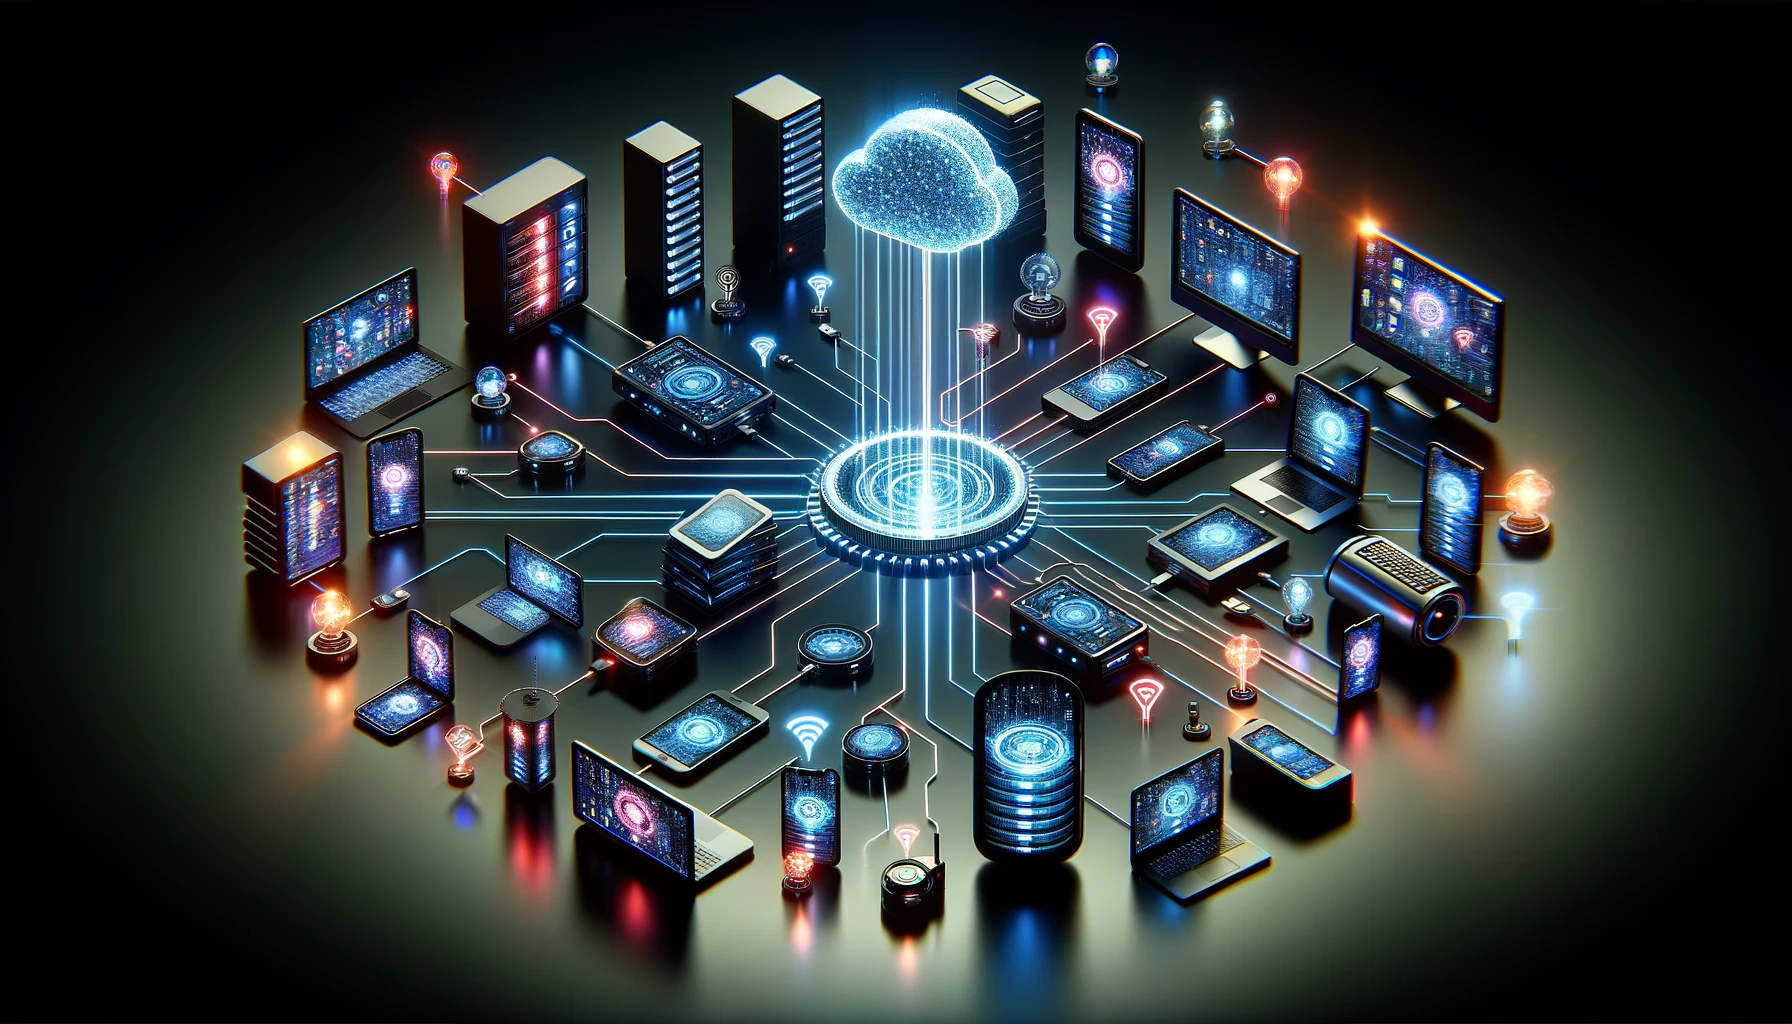
\includegraphics[width=1\textwidth]{content/1-relational-databases/figures/i1-databases-everywhere.png}
    \caption{A system of databases and services}
    \label{fig:0.i1-databases-everywhere.png}
\end{figure}

You interact every day with devices that include databases, and with services that does the same. Examples are:

\begin{itemize}
    \item Your phone and every single app on your phone
    \item Your computer and most of the applications herein.
    \item All websites you visit, such as your bank, google, etc. (few exceptions exist, but any website that is dynamic and that can save data, will most likely also use a database)
    \item Your social media
    \item Your email
    \item Your favorite online store
    \item Your favorite games
\end{itemize}

While databases are everywhere now, this was not always the case. Databases have been around for a long time, but they were not always as popular as they are now. The first databases were created in the 1960s, and were used for large scale data processing, while they slowly became more and more used, expecially at the end of 1970, and the beginning of 1980. The first relational database was created in 1970, and was called the relational model. It was created by Edgar F. Codd, and was based on the mathematical theory of sets and relations. The relational model was a huge success, and is still the most widely used database model today. The relational model was so successful, that it is often used as a synonym for relational databases, and that relational databases are often called relational models.

Initially, relational databases were predominantly utilized in substantial organizations such as banks, or for calculating salaries in major corporations. This exclusivity was due to the high cost of the computers required to operate these databases, rendering them unaffordable for the average person. However, this scenario transformed dramatically in the 1980s with the rising popularity and affordability of personal computers. As computers became more accessible, a larger segment of the population could afford to own and run a database on their personal computers. Consequently, this led to a surge in database usage, significantly increasing the demand for and creation of databases. The growth in demand meant that an ever-increasing number of people began to use databases, further amplifying their prevalence and importance in the digital world.

\section{What is SQL?}
SQL, which stands for Structured Query Language, is the cornerstone of relational databases. It's a specialized programming language designed for managing and manipulating data held in a relational database management system (RDBMS). SQL is essential for various operations within these databases, including querying, updating, and managing data.

Relational databases store data in tables, which are akin to spreadsheets with rows and columns. Each row represents a unique record, and each column a specific attribute of the data. The power of relational databases lies in their ability to efficiently organize and retrieve large volumes of data through the use of relations, typically in the form of tables.

SQL plays a pivotal role in this process. It allows users to:

\begin{itemize}
\item \textbf{Query Data:} SQL can retrieve specific data from a database through queries. For instance, if you want to find all customers from a particular city, SQL can quickly filter and display this information.
\item \textbf{Insert and Update Data:} Adding new records or updating existing ones is straightforward with SQL. It ensures data accuracy and integrity while modifying the database.
\item \textbf{Create and Modify Schema:} SQL is used to create the database structure, like tables, and modify it as needed. This includes defining the columns, data types, and constraints.
\item \textbf{Data Manipulation:} Beyond basic queries, SQL can perform complex data manipulations, combining data from multiple tables and executing sophisticated analytical functions.
\end{itemize}

One of SQL's greatest strengths is its widespread adoption and standardization. Most relational database systems use SQL, making it a crucial skill for database professionals. Its syntax and commands are relatively consistent across different database systems, with only minor variations. Understanding SQL is fundamental for anyone looking to work with relational databases, as it opens the door to efficiently managing and utilizing vast sets of data in an organized manner.

\section{What is PostgreSQL?}
PostgreSQL, often simply called Postgres, is an advanced, open-source relational database management system (RDBMS) that stands out in the vast landscape of relational databases. It's renowned for its robustness, scalability, and alignment with SQL standards. Understanding PostgreSQL in the context of relational databases involves appreciating its unique features and the reasons behind its popularity.

\begin{figure}[h]
    \centering
    
\includegraphics[width=0.4\textwidth]{content/1-relational-databases/figures/PostgreSQL_logo.3colors.540x557.png}
    \caption{PostgreSQL Logo}
    \label{fig:PostgreSQL_logo.3colors.540x557.png}
\end{figure}

Choosing PostgreSQL for database management comes with several advantages:

\begin{itemize}
    \item \textbf{Open Source:} Being open-source, it's free to use, modify, and distribute. This aspect makes it particularly attractive for startups and companies looking to reduce costs without sacrificing quality.
    \item \textbf{Community-Driven Development:} PostgreSQL benefits from a vibrant community that continuously contributes to its development, ensuring the database is always evolving to meet user needs.
    \item \textbf{Reliability and Stability:} It's known for its data integrity and resilience. Businesses can rely on PostgreSQL for critical applications requiring consistent uptime and robustness.
    \item \textbf{Flexibility for Developers:} PostgreSQL's support for various programming languages and its extensibility make it highly adaptable for a wide range of applications.
    \item \textbf{Scalability:} It handles large volumes of data effectively, making it suitable for businesses that anticipate growth in data volume and user load.
\end{itemize}

PostgreSQL represents a sophisticated and reliable choice within the realm of relational databases. Its adherence to SQL standards, coupled with its open-source nature, makes it a formidable tool for businesses and developers seeking a powerful, scalable, and cost-effective database solution. The most used relational database management systems are currently Oracle, MySQL (Hereunder MariaDB and other variants), Microsoft SQL Server, PostgreSQL, IBM Db2, and SQLite.

This book currently uses PostgreSQL, but will later add examples in MySQL (or variants), MSSQL and SQLite.


\section{Getting to terms with the terminology}
Understanding the realm of database systems requires familiarity with several core terminologies. Let's delve into each of these terms and explore their interrelationships.

\subsection{Overall Database Terms}
The terms one needs to understand, and how they relate to each other, are shown in \cref{fig:1.dbms-definitions.png}.

\begin{figure}[h]
    \centering
    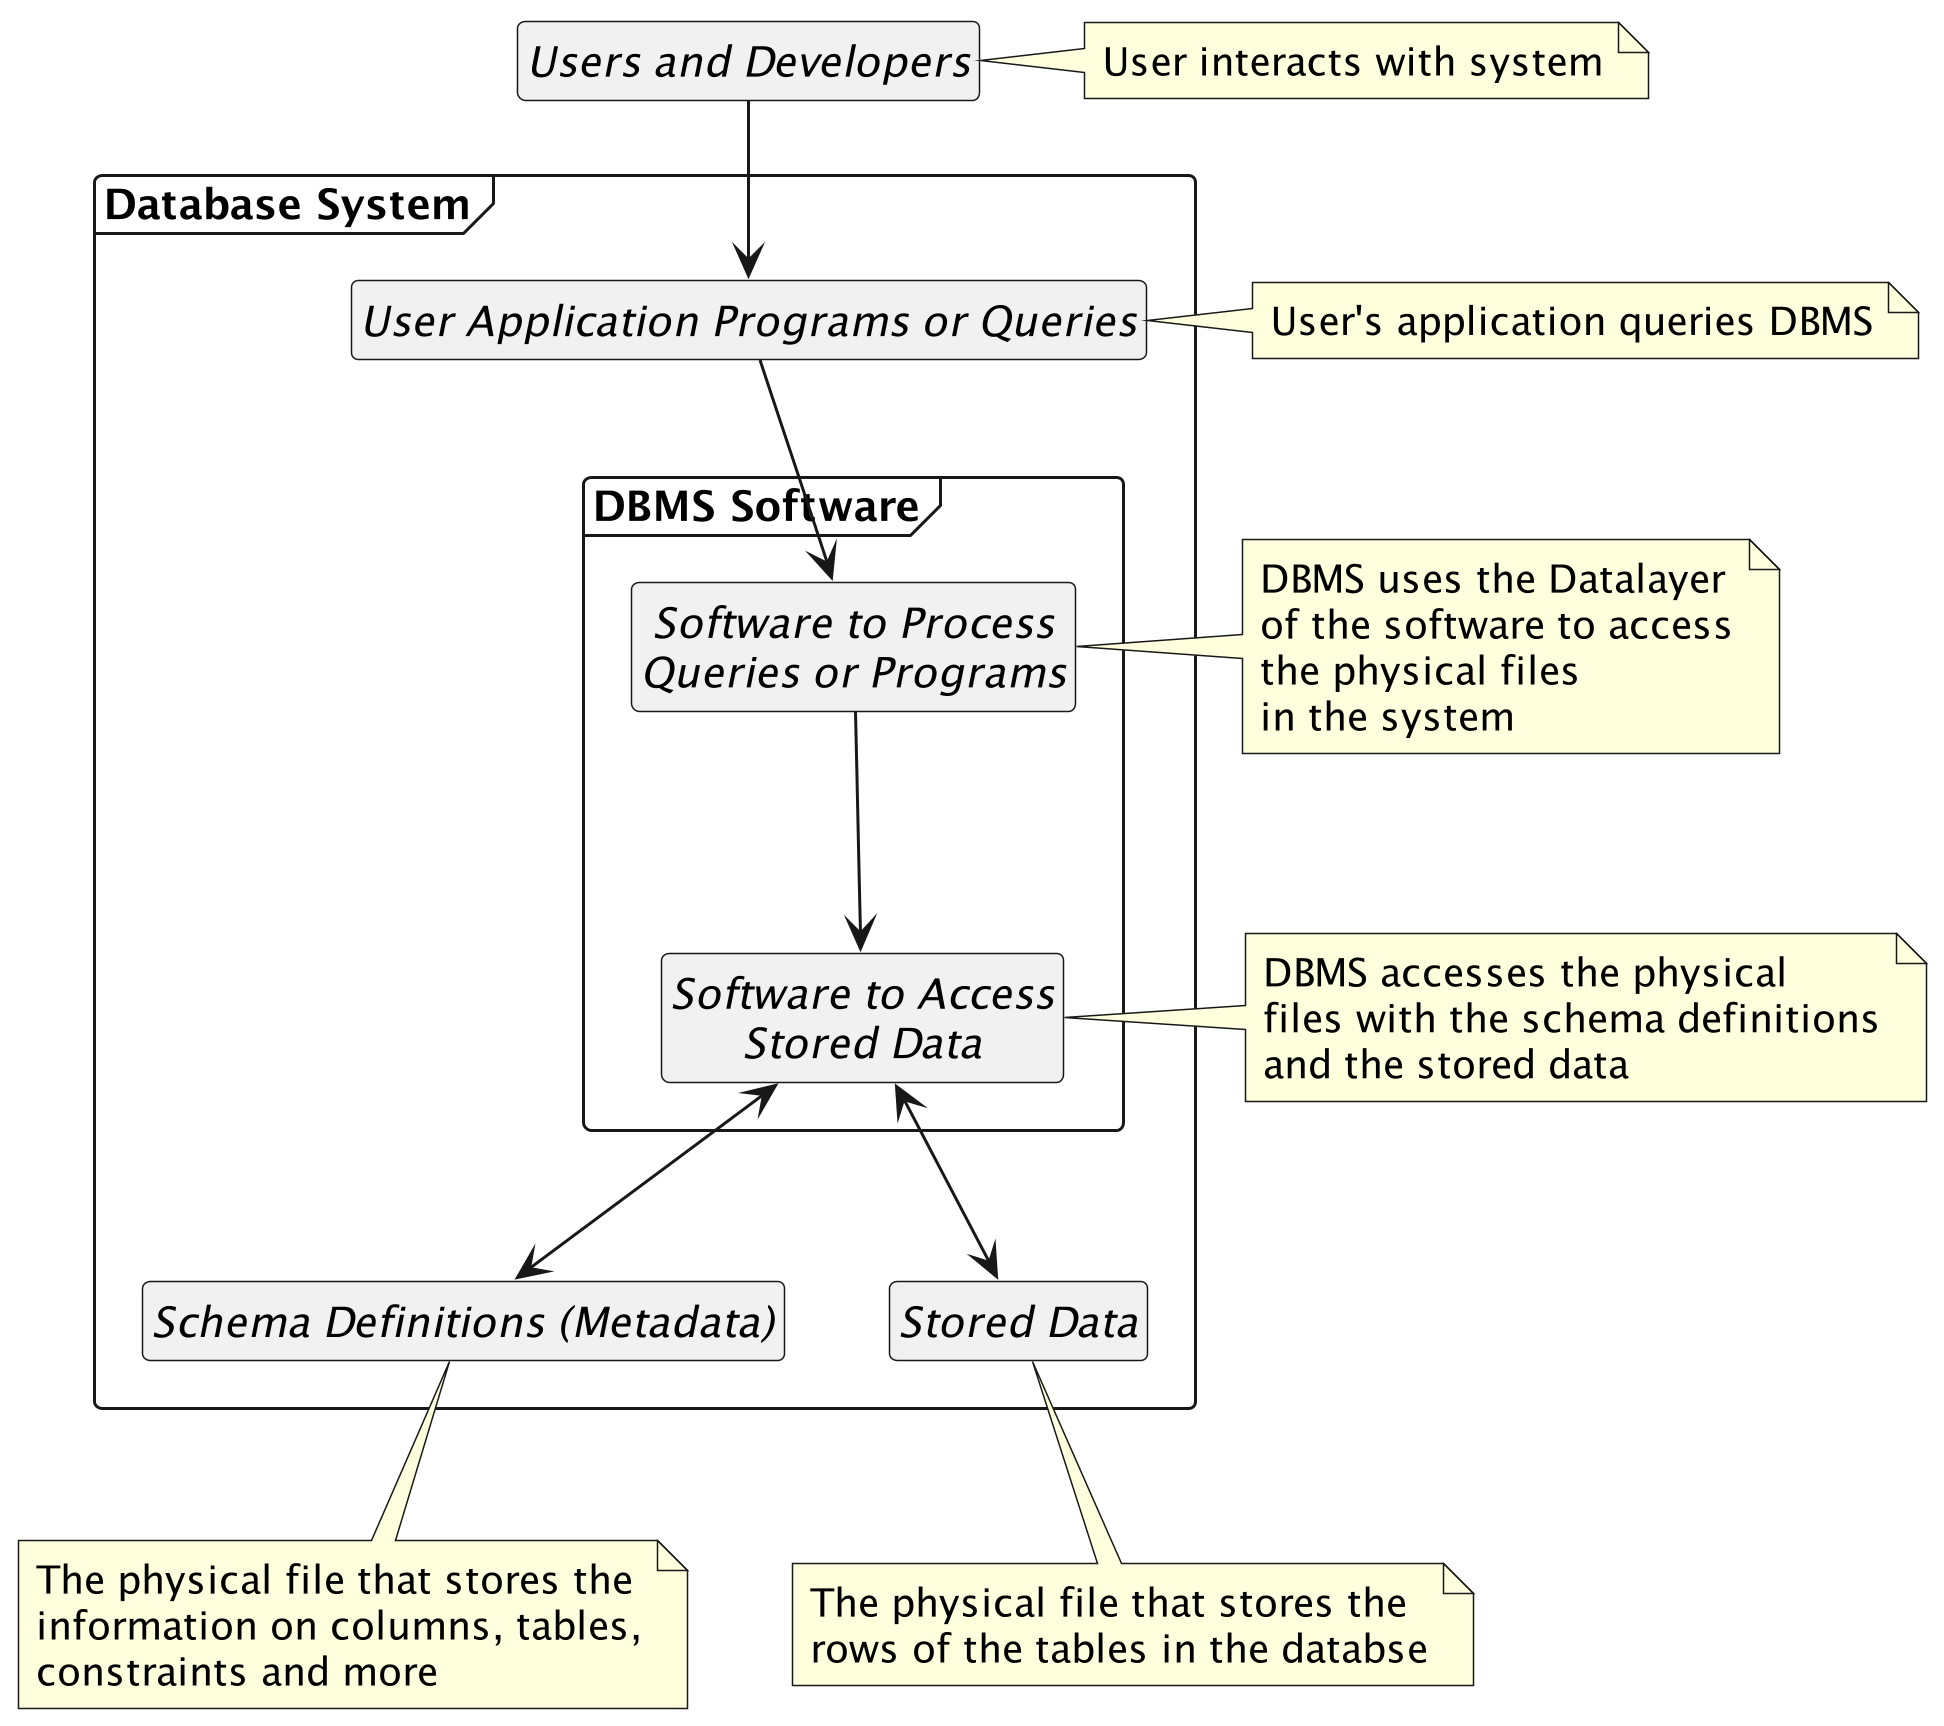
\includegraphics[width=1\textwidth]{content/1-relational-databases/figures/1.dbms-definitions.png}
    \caption{High Level Explanation of a Database Management System}
    \label{fig:1.dbms-definitions.png}
\end{figure}

\begin{enumerate}
    \item \textbf{Database Systems:} A Database System is an integrated set of software tools that allows users to store, modify, and extract information from a database. It encompasses the DBMS software, the database itself (which includes the schema definitions and stored data), and the user application programs or queries.
    \item \textbf{User Application Programs or Queries:} User Application Programs or Queries refer to the software and commands that interact with the database system. These can range from simple query commands in SQL to complex programs written in programming languages like Python, Java, or C#, designed to manipulate or retrieve data from the database.
    \item \textbf{DBMS Software:} DBMS Software, or Database Management System Software, is the core component of a database system. It acts as an intermediary between the user and the database. The DBMS manages the stored data, ensuring its integrity, security, and consistency. It also handles tasks such as data retrieval, update, and administration.
    \item \textbf{Schema Definitions:} Schema Definitions in a database system represent the logical structure of the entire database. They define how data is organized and how the relationships among different data elements are established. The schema includes definitions for tables, columns, data types, constraints, and relationships. It's like a blueprint for the database, dictating its organization and how the data within it is related.
    \item \textbf{Stored Data:} Stored Data is the actual data that resides in the database. This is the collection of information that has been stored in accordance with the schema definitions. Stored data can include various types of data, such as textual data, numerical data, dates, or binary data, depending on the nature of the database and its schema.
\end{enumerate}


The relationship among these components is hierarchical and interdependent:

- At the base, we have the \textbf{Stored Data}, which is the essence of the database.
- This data is structured and organized according to the \textbf{Schema Definitions}.
- The \textbf{DBMS Software} serves as the mediator between the stored data and the end-users. It uses the schema definitions to ensure data is correctly stored and retrieved.
- \textbf{User Application Programs or Queries} interact with the DBMS software to perform operations on the data — whether it's querying for specific information, updating records, or performing analyses.
- All these components together constitute the \textbf{Database System}, which is the overall environment enabling data management and utilization.

\subsection{The anatomy of a table}

\begin{figure}[h]
    \centering
    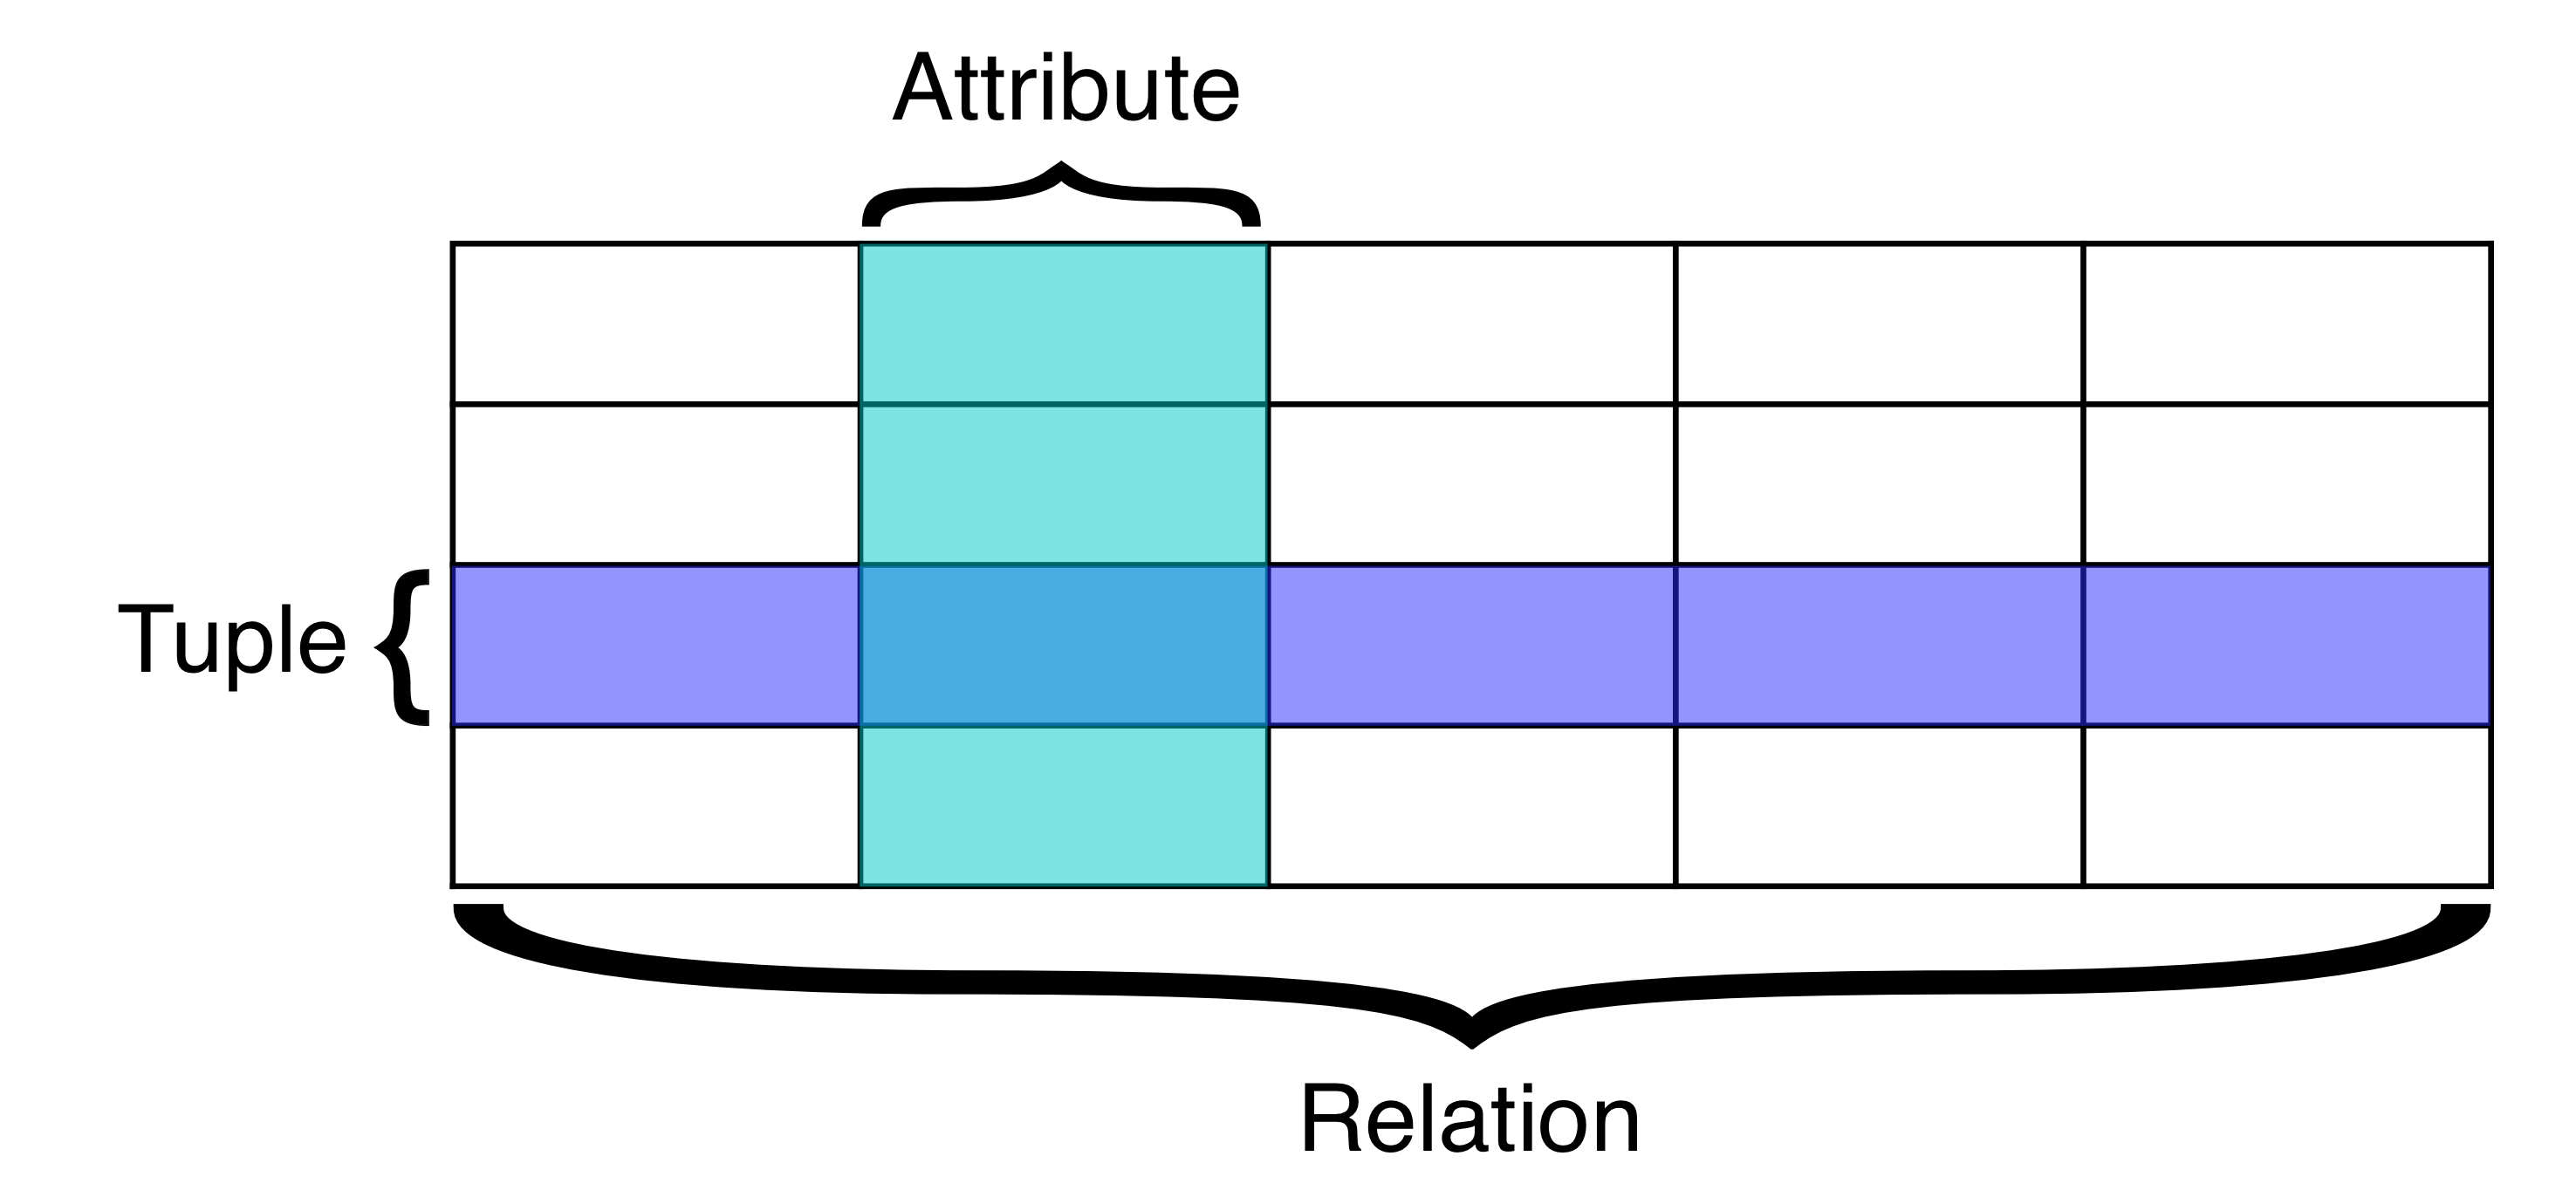
\includegraphics[width=0.8\textwidth]{content/1-relational-databases/figures/2.table-definitions.png}
    \caption{Table Terminology (Artist: Chris Martin)}
    \label{fig:2.table-definitions.png}
\end{figure}

\section{Getting Started}


% ******************************* Chapter: Relational Database Basics ****************************
\chapter{Relational Database Basics}
\label{chap:relational:relational-database-basics}
This chapter contains the basic building blocks to get started with basic relational databases.

\section{Creating your first database}

\section{Managing Databases}

\subsection{Creating a database}
\begin{minted}[fontsize=\footnotesize]{postgresql}
    -- Creating a database with full syntax
    CREATE DATABASE database_name
    WITH
        [OWNER =  role_name]
        [TEMPLATE = template]
        [ENCODING = encoding]
        [LC_COLLATE = collate]
        [LC_CTYPE = ctype]
        [TABLESPACE = tablespace_name]
        [ALLOW_CONNECTIONS = true | false]
        [CONNECTION LIMIT = max_concurrent_connection]
        [IS_TEMPLATE = true | false ]
\end{minted}

\begin{minted}[fontsize=\footnotesize]{postgresql}
    -- Creating an ACME database with minimal syntax
    CREATE DATABASE Acme;
\end{minted}

\begin{minted}[fontsize=\footnotesize]{postgresql}
    -- Creating a ACME database with enabled options
    CREATE DATABASE Acme 
    WITH
        OWNER = postgres
        CONNECTION LIMIT = 50;
        IS_TEMPLATE = false;
\end{minted}

\subsection{Altering a database}
\begin{minted}[fontsize=\footnotesize]{postgresql}
    -- Create a table
    CREATE TABLE tableName (
        tableName_id SERIAL PRIMARY KEY, -- auto incrementing id
        username VARCHAR (50) UNIQUE NOT NULL, -- unique username
        password VARCHAR (250) NOT NULL -- never store in plain text
    );
\end{minted}

\subsection{Deleting a database}
\begin{minted}[fontsize=\footnotesize]{postgresql}
    -- Create a table
    CREATE TABLE tableName (
        tableName_id SERIAL PRIMARY KEY, -- auto incrementing id
        username VARCHAR (50) UNIQUE NOT NULL, -- unique username
        password VARCHAR (250) NOT NULL -- never store in plain text
    );
\end{minted}

\subsection{Switch databases}
\begin{minted}[fontsize=\footnotesize]{sql}
    /* Change to database_name
     * This does not work with PostgreSQL */
    USE database_name;
\end{minted}

\begin{minted}[fontsize=\footnotesize]{psql}
    -- Change to database_name from psql command line
    \connect database_name
\end{minted}


\section{Managing Tables}

\subsection{Creating tables}
\begin{minted}[fontsize=\footnotesize]{postgresql}
    -- Create a table
    CREATE TABLE tableName (
        tableName_id SERIAL PRIMARY KEY, -- auto incrementing id
        username VARCHAR (50) UNIQUE NOT NULL, -- unique username
        password VARCHAR (250) NOT NULL -- never store in plain text
    );
\end{minted}

\begin{minted}[fontsize=\footnotesize]{postgresql}
    -- Create account table
    CREATE TABLE account (
        id serial PRIMARY KEY,
        username VARCHAR (50) UNIQUE NOT NULL,
        created_on TIMESTAMP NOT NULL, 
        last_login TIMESTAMP
    );
    
    /* Create blog entries table
     * the created_by column references the 
     * id column in the account table */
    CREATE TABLE blog_entries (
        id serial PRIMARY KEY, 
        header VARCHAR (255) NOT NULL,
        body TEXT NOT NULL,
        created_by INTEGER NOT NULL REFERENCES account (id)
    );
\end{minted}

\subsection{Altering tables}
\begin{minted}[fontsize=\footnotesize]{postgresql}
    -- Create a table
    CREATE TABLE account (
        user_id SERIAL PRIMARY KEY,
        username VARCHAR (50) UNIQUE NOT NULL,
        password VARCHAR (50) NOT NULL,
        email VARCHAR (355) UNIQUE NOT NULL,
        created_on TIMESTAMP NOT NULL,
        last_login TIMESTAMP
    );
\end{minted}

\subsection{Deleting tables}
\begin{minted}[fontsize=\footnotesize]{postgresql}
    -- Create a table
    CREATE TABLE account (
        user_id SERIAL PRIMARY KEY,
        username VARCHAR (50) UNIQUE NOT NULL,
        password VARCHAR (50) NOT NULL,
        email VARCHAR (355) UNIQUE NOT NULL,
        created_on TIMESTAMP NOT NULL,
        last_login TIMESTAMP
    );
\end{minted}

\section{CRUD Operations}

\section{Joins and querying related tables}

% ******************************* Chapter: ER, EER Modeling and Database Design ****************************
\chapter{ER, EER Modeling and Database Design}
\label{chap:relational:eer-modeling-and-database-design}
This chapter teaches basic ER and ER modelling, and how to design a database from an ER model.

\section{The purpose of ER and EER modeling}
\section{Diagram Elements}
\section{ER versus EER modeling}
\section{Mapping to tables}

% ******************************* Chapter: Database Normalization ****************************
\chapter{Database Normalization}
\label{chap:relational:database-normalization}
This chapter teaches database normalization to the 4th normal form.

\section{What is database normalization?}
\section{Shorthand techniques}
\section{First normal form}
\section{Second normal form}
\section{Third normal form}
\section{Fourth normal form}
\section{Normalization of other formats}

% ******************************* Chapter: Advanced Relational Databases ****************************
\chapter{Advanced Relational Databases}
\label{chap:relational:advanced-relational-databases}
This chapter teaches advanced relational database concepts.

\section{Transactions}
\section{Indexes}
\section{Views}
\section{Stored Procedures}
\section{Triggers}
\section{User Defined Functions}
\section{Security}
\section{Performance Tuning}


